%% Based on a TeXnicCenter-Template by Tino Weinkauf.
%%%%%%%%%%%%%%%%%%%%%%%%%%%%%%%%%%%%%%%%%%%%%%%%%%%%%%%%%%%%%

%%%%%%%%%%%%%%%%%%%%%%%%%%%%%%%%%%%%%%%%%%%%%%%%%%%%%%%%%%%%%
%% HEADER
%%%%%%%%%%%%%%%%%%%%%%%%%%%%%%%%%%%%%%%%%%%%%%%%%%%%%%%%%%%%%
\documentclass[a4paper,twoside,10pt]{report}
% Alternative Options:
%	Paper Size: a4paper / a5paper / b5paper / letterpaper / legalpaper / executivepaper
% Duplex: oneside / twoside
% Base Font Size: 10pt / 11pt / 12pt


%% Language %%%%%%%%%%%%%%%%%%%%%%%%%%%%%%%%%%%%%%%%%%%%%%%%%
%\usepackage[USenglish]{babel} %francais, polish, spanish, ...
\usepackage[dutch]{babel}
\usepackage[T1]{fontenc}
\usepackage[ansinew]{inputenc}

\usepackage{lmodern} %Type1-font for non-english texts and characters


%% Packages for Graphics & Figures %%%%%%%%%%%%%%%%%%%%%%%%%%
\usepackage{graphicx} %%For loading graphic files
%\usepackage{subfig} %%Subfigures inside a figure
%\usepackage{pst-all} %%PSTricks - not useable with pdfLaTeX

%% Please note:
%% Images can be included using \includegraphics{Dateiname}
%% resp. using the dialog in the Insert menu.
%% 
%% The mode "LaTeX => PDF" allows the following formats:
%%   .jpg  .png  .pdf  .mps
%% 
%% The modes "LaTeX => DVI", "LaTeX => PS" und "LaTeX => PS => PDF"
%% allow the following formats:
%%   .eps  .ps  .bmp  .pict  .pntg


%% Math Packages %%%%%%%%%%%%%%%%%%%%%%%%%%%%%%%%%%%%%%%%%%%%
\usepackage{amsmath}
\usepackage{amsthm}
\usepackage{amsfonts}


%% Line Spacing %%%%%%%%%%%%%%%%%%%%%%%%%%%%%%%%%%%%%%%%%%%%%
%\usepackage{setspace}
%\singlespacing        %% 1-spacing (default)
%\onehalfspacing       %% 1,5-spacing
%\doublespacing        %% 2-spacing


%% Other Packages %%%%%%%%%%%%%%%%%%%%%%%%%%%%%%%%%%%%%%%%%%%
%\usepackage{a4wide} %%Smaller margins = more text per page.
%\usepackage{fancyhdr} %%Fancy headings
\usepackage{longtable} %%For tables, that exceed one page
\usepackage{hyperref}
\usepackage{booktabs}


%%%%%%%%%%%%%%%%%%%%%%%%%%%%%%%%%%%%%%%%%%%%%%%%%%%%%%%%%%%%%
%% Remarks
%%%%%%%%%%%%%%%%%%%%%%%%%%%%%%%%%%%%%%%%%%%%%%%%%%%%%%%%%%%%%
%
% TODO:
% 1. Edit the used packages and their options (see above).
% 2. If you want, add a BibTeX-File to the project
%    (e.g., 'literature.bib').
% 3. Happy TeXing!
%
%%%%%%%%%%%%%%%%%%%%%%%%%%%%%%%%%%%%%%%%%%%%%%%%%%%%%%%%%%%%%

%%%%%%%%%%%%%%%%%%%%%%%%%%%%%%%%%%%%%%%%%%%%%%%%%%%%%%%%%%%%%
%% Options / Modifications
%%%%%%%%%%%%%%%%%%%%%%%%%%%%%%%%%%%%%%%%%%%%%%%%%%%%%%%%%%%%%

%\input{options} %You need a file 'options.tex' for this
%% ==> TeXnicCenter supplies some possible option files
%% ==> with its templates (File | New from Template...).



%%%%%%%%%%%%%%%%%%%%%%%%%%%%%%%%%%%%%%%%%%%%%%%%%%%%%%%%%%%%%
%% DOCUMENT
%%%%%%%%%%%%%%%%%%%%%%%%%%%%%%%%%%%%%%%%%%%%%%%%%%%%%%%%%%%%%
\begin{document}

\pagestyle{empty} %No headings for the first pages.


%% Title Page %%%%%%%%%%%%%%%%%%%%%%%%%%%%%%%%%%%%%%%%%%%%%%%
%% ==> Write your text here or include other files.

%% The simple version:
%\title{Verslag Multimedia: modelleren en programmeren}
%\author{Joris Schelfaut}
%\date{} %%If commented, the current date is used.
%\maketitle

\begin{titlepage}
%\begin{center}


\includegraphics[height=.15\textheight,width=.50\textwidth]{data/kuleuven.png}\\[3cm]

	%\begin{center}
		%\Huge $\rvert$ G0Q55A $\vert$ \\
		\begin{center}
		\Huge Verslag Multimedia: modelleren en programmeren \\ [.5 cm]
		
		\LARGE Het ontwikkelen van een mobiele applicatie in Android en iOS \\ [.5 cm]
		\LARGE Joris Schelfaut	\\ [5 cm]
		\end{center}
		\large G0Q55A - Multimedia: modelleren en programmeren	\\
		\large Prof. ir. E. Duval	\\
		\large 2012-2013	\\ [1 cm]
	%\end{center}
	\vfill

% Bottom of the page
%{\large 2012-2013}\\
%{\large G0Q55A - Multimedia: modelleren en programmeren}\\
%{\large Prof. ir. E. Duval}
%\end{center}
\end{titlepage}

%\pagebreak

%% The nice version:
%\input{titlepage} %%You need a file 'titlepage.tex' for this.
%% ==> TeXnicCenter supplies a possible titlepage file
%% ==> with its templates (File | New from Template...).


%% Inhaltsverzeichnis %%%%%%%%%%%%%%%%%%%%%%%%%%%%%%%%%%%%%%%
\tableofcontents %Table of contents
\cleardoublepage %The first chapter should start on an odd page.

\pagestyle{plain} %Now display headings: headings / fancy / ...



%% Chapters %%%%%%%%%%%%%%%%%%%%%%%%%%%%%%%%%%%%%%%%%%%%%%%%%

% introductie 0.5 blz
\chapter{Introductie}\label{chapter:introductie}

Dit is het eindverslag voor de cursus 'Multimedia: modelleren en pogrammeren'. Het doel van deze cursus is om een mobiele applicatie te ontwerpen en implementeren in verschillende technologi\"en (iOS, Android, HTML5, ...) om uiteindelijk inzicht te verwerven in de sterktes en zwaktes van deze technologi\"en.

De applicatie is een Quantified Self App. Dit soort toepassing vraagt de gebruiker om invoer, en/of verzamelt deze automatisch afhankelijk van het type data, gedurende een zekere periode. Deze data kan dan gevisualiseerd worden om mogelijk gedragspatronen te onthullen\cite{govaerts2012}.

De technologie\"en die worden besproken in dit verslag zijn iOS en Android. Alle code voor dit project is open source en kan gevonden en gedownloaded worden van github\footnote{\url{https://github.com/JorisSchelfaut/mumedev}}. Naast dit verslag kan informatie over het project gevonden worden op de wordpress blog\footnote{\url{http://mumedev.wordpress.com/}} en youtube vlog\footnote{\url{http://www.youtube.com/user/mumedev}}.

We bespreken eerst het idee achter de applicatie. Vervolgens kijken we naar een scenario en daarna naar het storyboard van de applicatie. Dan wordt de architectuur en het software ontwerp van de applicatie voor de verschillende technologie\"en bekeken. Hierna maken we een vergelijking tussen de verschillende technologie\"en. We eindigen met een besluit.

% 0.5 blz
\chapter{Idee}\label{chapter:idee}

De applicatie die we zullen ontwerpen en implementeren is een Quantified Self applicatie getiteld 'Moggle', een woordspeling op 'mood' en 'Toggl'. Het basisidee was om de werkuren die gepresteerd werden door de gebruiker manueel te laten ingeven, of indien mogelijk automatisch laten importeren via Toggle, en vervolgens zijn prestaties te laten evalueren volgens drie indicatoren: slecht, gemiddeld en goed. Ten slotte geeft de gebruiker zijn gemoedstoestand in. Het resultaat is dus een datamodel waarin de werkkwantiteit en -kwaliteit aan de gemoedstoestand gekoppeld worden.

Uitbreidingen hierop zouden kunnen zijn om ook het tijdstipaspect in rekening te brengen (e.g. dag van de week), werklocatie, achtergrondgeluiden tijdens het werk, de specifieke activiteit (studeren, programmeren, trainen, ...) en dergelijke meer. Het automatisch 'tracken' van zulke parameters is waarschijnlijk niet eenvoudig, aangezien het toestel niet noodzakelijk aanstaat tijdens het presteren van de uren zelf.

% scenario 0.5 blz
\chapter{Scenario}\label{chapter:scenario}

We beschrijven een kort scenario van een persoon die de applicatie gebruikt om na te gaan of er een correlatie zou kunnen bestaan tussen zijn geleverde werk en zijn gemoedstoestand.\\

%{\addtolength{\leftskip}{5mm} ...text... }

Het is maandag. Een student heeft net een vijftal uren aan een verslag gewerkt. Hij houdt het voor bekeken voor die dag en vult zijn gepresteerde uren in op de Moggle applicatie, en ook de rating van zijn werk en zijn gemoedstoestand. Hij is tevreden over zijn werk en geeft zijn gemoedstoestand een rating van 9 op 10.

Woensdag, donderdag en zaterdag speelt zich eenzelfde scenario af met respectievelijk 2, 5 en 7 uren gewerkt, 'slecht', 'goed' en 'matig' als werkkwaliteit en 3, 7 en 7 als ratings voor zijn gemoedstoestand.

Wanneer hij zijn resultaten bekijkt, merkt hij dat slecht en weinig werk leveren doorgaans correleert met een slechte gemoedstoestand, terwijl goed werk leveren vooral overeenstemt met een goede gemoedstoestand. Veel en goed werk leveren lijkt echter niet altijd te correleren met een goede gemoedstoestand.


% storyboard 1 bladzijde
\chapter{Storyboard}\label{chapter:storyboard}

Het volledige storyboard is te zien op figuur \ref{fig:storyboard}. Het storyboard bestaat uit drie fases:

\begin{enumerate}
	\item In de eerste stap heeft de gebruiker de keuze de resultaten te bekijken of om een nieuwe data in te geven.
	\item De optie 'start' brengt de gebruiker naar het eerste invoerscherm. De gebruiker kan nu het aantal uren ingeven dat hij/zij heeft gepresteerd en een rating geven betreffende de kwaliteit van deze prestatie.
	\item Via de optie 'next' komt gebruiker in het laatste scherm terecht. Hier geeft de gebruiker een kwantificatie van zijn gemoedstoestand in op een schaal van $1$ tot $10$.
\end{enumerate}

% http://en.wikibooks.org/wiki/LaTeX/Importing_Graphics
\begin{figure}
  \begin{center}
  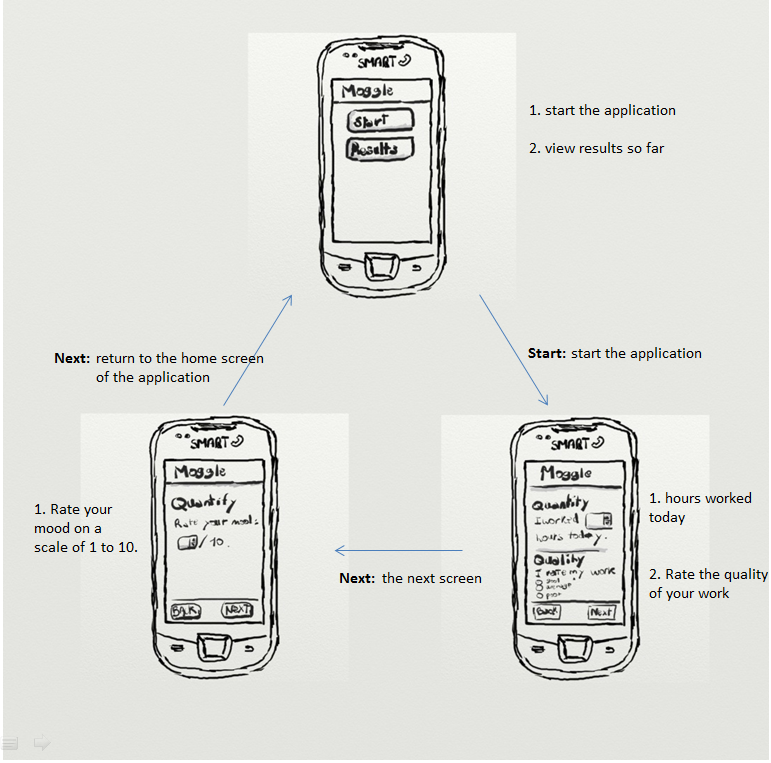
\includegraphics[scale=0.6]{data/storyboard-final}
	\end{center}
  \caption{Moggle storyboard}
	\label{fig:storyboard}
\end{figure}


% Architectuur 1 blz
\chapter{Architectuur}\label{chapter:architectuur}

%%%%%%%%%%%%%%%%%%
% SECTION
%%%%%%%%%%%%%%%%%%
\section{Verzamelen van data}\label{section:manuele_datainvoer}

Om relatief snel een applicatie te kunnen implementeren, werd in de applicatie eerst manuele datainvoer voorzien.

Het aanvankelijke idee om gebruik te maken van de Toggle API\footnote{\url{https://www.toggl.com/public/api}} is uiteindelijk niet meer ge\"implementeerd. Indien de gebruik zou gemaakt worden van de Toggl API zou er natuurlijk een internetconnectie moeten opgezet worden. De gebruiker zou zich moeten authenticeren, waarna logingegevens in lokaal zouden kunnen bijgehouden worden en dergelijke.


%%%%%%%%%%%%%%%%%%
% SECTION
%%%%%%%%%%%%%%%%%%
\section{Opslag van data}\label{section:local_storage}

De applicatie maakt gebruik van lokale opslag om gegevens te persisteren. De records bevatten relatief beperkte, numerieke informatie. De huidige smartphones hebben gemakkelijk meer dan een gigabyte aan intern geheugen\cite{schiesser2012}, dus de gebruiker zou al duizenden records moeten opslaan vooraleer een significant deel van de opslagcapaciteit zou gebruikt worden. Daarnaast heeft lokale opslag het voordeel dat het een hogere beschikbaarheid aanbiedt dan opslag op een externe server. Ten slotte is externe, online opslag geen vereiste om resultaten te verkrijgen die significant zijn. Uiteraard kan het vergelijken met andere gebruikers, gemiddeldes en uitschieters een interessante uitbreiding zijn bij de data-analyse.

De interne architectuur van de applicatie is afgebeeld op figuur \ref{fig:architecture}.

\begin{figure}
  \begin{center}
  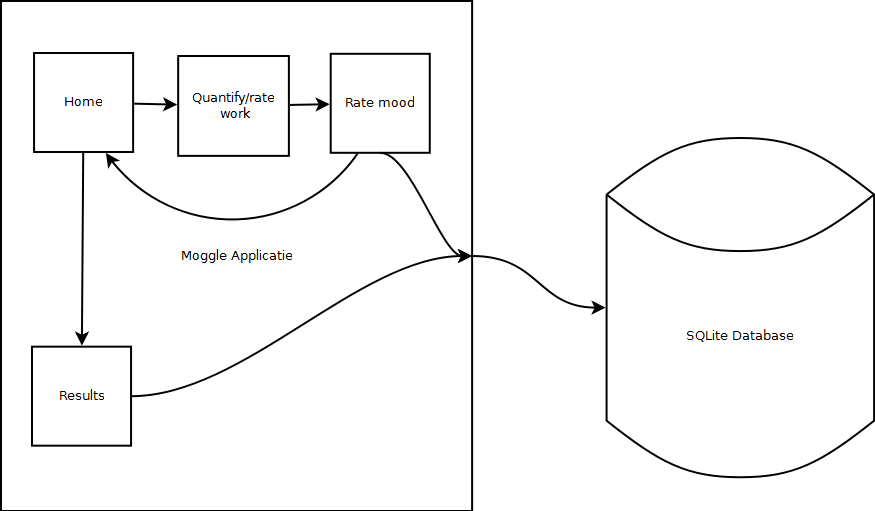
\includegraphics[scale=0.35]{data/internal-architecture}
	\end{center}
  \caption{Interne architectuur van de Moggle applicatie}
  \label{fig:architecture}
\end{figure}

%Een cli\"ent-server model 






% Software ontwerp
\chapter{Softwareontwerp}\label{chapter:softwareontwerp}


%%%%%%%%%%%%%%%%%%%%%%%%%%%%%%%%%%%%%%%%%%%%%%
% SECTION Data model
%%%%%%%%%%%%%%%%%%%%%%%%%%%%%%%%%%%%%%%%%%%%%%
\section{Datamodel}\label{section:data_model}

Beide applicaties maken gebruik van hetzelfde datamodel. Het is een eenvoudige tabel in een SQLite database zoals te zien in tabel \ref{tab:qdat}. SQLite is relatief eenvoudig te integreren in beide technologie\"en\footnote{SQLite tutorial voor iOS: \cite{techotopia2012sqlite}, SQLite tutorial voor Android: \cite{android2013sqlite}}. De SQL-code om een database en tabellen aan te maken en te verwijderen is uiteraard hetzelfde.

\begin{table}[h]
\caption{QDat SQLite Table}
\begin{center}
	\begin{tabular}{ l l } % l = left-aligned column
		\hline
		\textbf{QDat}		&									\\
		\hline
		id (pk)					&		INTEGER 			\\
		date 						&		TIMESTAMP 		\\
		work\_quantity	&		REAL[0, 24]		\\
		work\_quality		&		INTEGER[0..2]	\\
		mood\_quantity	&		REAL[0, 10]		\\
		\hline
	\end{tabular}
\end{center}
\label{tab:qdat}
\end{table}

Een andere mogelijkheid, specifiek voor iOS, is het gebruik van Core Data. Met dit framework kan dataopslag gebeuren aan de hand van een object-geori\"enteerde abstractielaag\cite{techotopia2012coredata}. Voor deze relatief kleine applicatie volstaat een SQLite database echter.



%%%%%%%%%%%%%%%%%%%%%%%%%%%%%%%%%%%%%%%%%%%%%%
% SECTION Structuur
%%%%%%%%%%%%%%%%%%%%%%%%%%%%%%%%%%%%%%%%%%%%%%
\section{Structuur}\label{section:structuur}

De projectstructuur voor de twee projecten verschilt weinig in grote lijnen. Het aantal schermen is hetzelfde, net als het aantal controllers. Het model voor de Android-applicatie is iets uitgebreider dan in de iOS-versie, maar dit is eerder een gevolg van de manier waarop de database werd ge\"implementeerd, dan de constraints van de technologie zelf.


%%%%%%%%%%%%%%%%%%%%
%			 Android
%%%%%%%%%%%%%%%%%%%%
\subsection{Android}

De Android-app is opgebouwd uit vier klassen die overerven van de \textit{Activity}-klasse, met bijbehorende XML-files voor de views zoals te zien in tabel \ref{tab:android_activities}. \textit{HomeActivity} is het startpunt van de applicatie. Het scherm toont twee knoppen: \'e\'en om te navigeren naar de \textit{QWorkActivity} pagina en \'e\'en om de resultatenpagina, \textit{DataVisActivity}, te laden. De view van \textit{QWorkActivity} bevat enkele labels, een invoerveld, een radioboxgroep en een knop om naar \textit{QMoodActivity} te navigeren. In de view van \textit{QMoodActivity} staat er een label, een slider en een knop om naar \textit{HomeActivity} terug te keren. Hierbij wordt eveneens de data gepersisteerd in de SQLite databank.

\begin{table}[h]
\caption{Android Activity klassen met bijbehorende XML-files}
\begin{center}
	\begin{tabular}{ l l } % l = left-aligned column
		\hline
		\textbf{Activity}								&	\textbf{XML}											\\
		\hline
		\textit{HomeActivity}.java			&	\textit{activity\_home}.xml 			\\
		\textit{QWorkActivity}.java			&	\textit{activity\_qwork}.xml			\\
		\textit{QMoodActivity}.java 		&	\textit{activity\_qmood}.xml 			\\
		\textit{DataVisActivity}.java		&	\textit{activity\_data\_vis}.xml	\\
		\hline
	\end{tabular}
\end{center}
\label{tab:android_activities}
\end{table}

Om de connectie met de database te maken, wordt er gebruik gemaakt van een implementatie van de SQLiteOpenHelper-klasse; de klasse \textit{DatabaseHandler} in dit project. De klasse \textit{CRUD<E>} is een templateklasse voor het beheren van een database tabel. Deze heeft de typische methodes \textit{createTable}, \textit{dropTable}, \textit{insert}, \textit{delete}, \textit{update} en \textit{select}.

De modelklasse \textit{QDat} implementeert de \textit{Parcelable} interface. Dit zorgt ervoor dat we op een effici\"ente manier objecten tussen \textit{Activity}-klassen kunnen doorgeven.

Het volledige klassediagram voor de Android-applicatie is te zien op figuur \ref{fig:android_classdiagram}.

\begin{figure}
  \begin{center}
  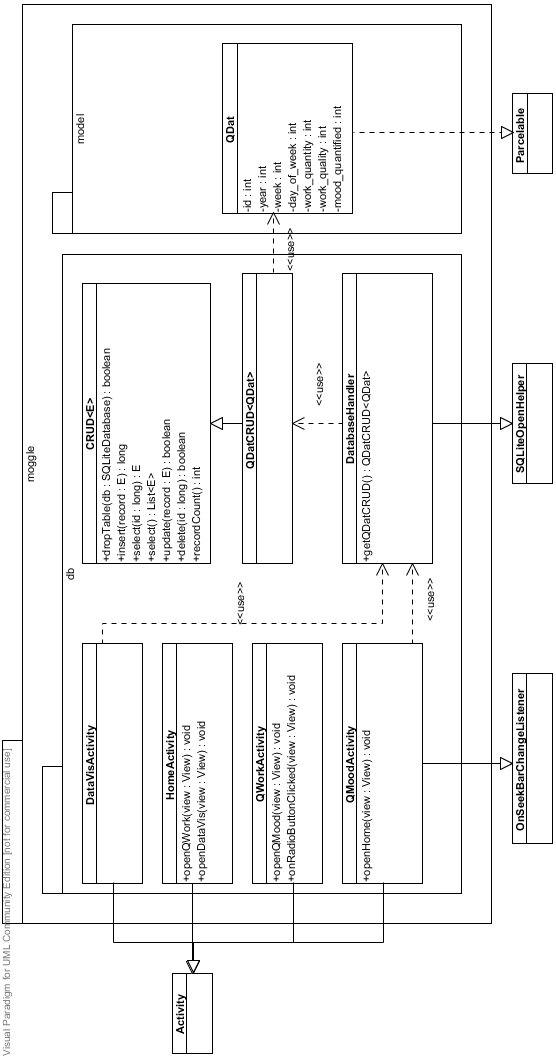
\includegraphics[scale=0.7]{data/diagram-android}
	\end{center}
  \caption{Android Class Diagram van de Moggle applicatie}
  \label{fig:android_classdiagram}
\end{figure}


%%%%%%%%%%%%%%%%
%			iOS
%%%%%%%%%%%%%%%%
\subsection{iOS}

Het ontwerpen van de iOS-app is grotendeels gebaseerd op het storyboard. Er zijn vier views met bijbehorende \textit{UIViewController}-implementaties: \textit{ViewController}, \textit{QWorkController}, \textit{QMoodController} en \textit{ResultsController}.

De UI-elementen komen grotendeels overeen met die van de Android-versie. Behalve in de view van de \textit{QWorkController}: de stepper biedt een mooie voorgedefinieerde functionaliteit om op een eenvoudige manier een natuurlijk getal in te geven door de huidige waarde met stappen van \'e\'en te verhogen of te verlagen.

Een interessante eigenschap van iOS is het doorgeven van argumenten tussen controllers van opeenvolgende views. Het volstaat hierbij in de methode \textit{prepareForSegue} de pointer naar het object expliciet te initialiseren in de targetcontroller.

Het klassediagram voor de iOS-applicatie is te zien op figuur \ref{fig:ios_classdiagram}. %Figuur \ref{fig:ios_storyboard} toont het storyboard van de iOS-applicatie.

\begin{figure}
  \begin{center}
  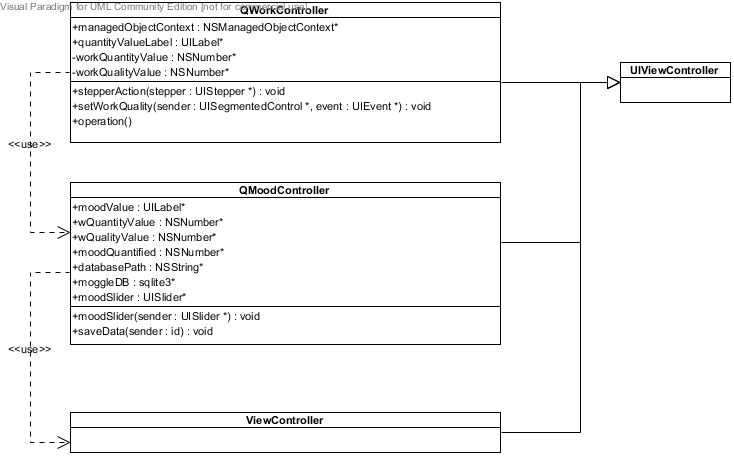
\includegraphics[scale=0.7]{data/diagram-ios}
	\end{center}
  \caption{iOS Class Diagram van de Moggle applicatie}
  \label{fig:ios_classdiagram}
\end{figure}

%\begin{figure}
%  \begin{center}
%  
\includegraphics[scale=0.7]{data/ios-storyboard}
%	\end{center}
%  \caption{iOS storyboard van de Moggle applicatie}
%  \label{fig:ios_storyboard}
%\end{figure}



%%%%%%%%%%%%%%%%%%%%%%%%%%%%%%%%%%%%%%%%%%%%%%
% SECTION Structuur
%%%%%%%%%%%%%%%%%%%%%%%%%%%%%%%%%%%%%%%%%%%%%%
\section{Uitbreidingen}\label{section:uibreidingen}

Mogelijke uitbreidingen aan de huidige applicaties zouden bijvoorbeeld de volgende kunnen zijn:

\begin{itemize}
	\item dataopslag gecentraliseerd op een server;
	\item	integratie met de Toggl API;
	\item	implementatie van verschillende data visualisaties;
	\item een notificatiesysteem uitbouwen op basis van gebruikersvoorkeuren;
	\item	combinatie met Google Calendar: afhankelijk van de weekplanning notificaties sturen;
	\item	...
\end{itemize}

Al bij al is het nog maar een zeer klein project, dus echt grote ontwerpbeslissingen hoefden nog niet genomen te worden. Door de applicatie enkel voor iPhone te ontwikkelen en niet voor bijvoorbeeld de iPad, worden bovendien een deel van de mogelijke problemen uitgesloten, gerelateerd aan de layout van de schermen en visualisaties.

% mogelijke uitbreidingen in de toekomst
% mogelijke veranderingen aan het huidige systeem











% 2 Bladijden
\chapter{Vergelijking technologie\"en}\label{chapter:vergelijking_technologieen}

% SECTION
\section{Properties}\label{section:properties_technologieen}

\subsection{Ondersteuning}

\subsubsection{Development Environment en simulator}

In termen van voorwaarden om van start te geraken in iOS en Android verschillen beide technologie\"en. Development in iOS is relatief gelimiteerd, Apple's IDE XCode is immers enkel beschikbaar op Mac OS platformen\cite{goadrich2011} en applicaties zoals Macincloud\footnote{\url{http://www.macincloud.com/}} waarmee een Mac services vanuit de browser kunnen worden gebruikt\cite{macincloud2013}, lijken nog niet echt op punt te staan, afgaande op eigen ervaring.

Daarentegen is Android development relatief toegankelijk. Dankzij de Java virtuele machine kan Eclipse op zowat elk platform ge\"installeerd worden samen met de Android Eclipse plugin\footnote{\url{http://developer.android.com/sdk/installing/installing-adt.html}}.

De Android simulator van Eclipse komt zeer log over, al zijn er kennelijk wel mogelijkheden om de performance te verbeteren\cite{stackoverflow2012}. De simulator voor iOS is wel zeer performant. Beide hebben het nadeel dat ze beperkt zijn voor het testen van bepaalde userinput; denk aan touch events, gebruik van acceleratiemeter en dergelijke\cite{goadrich2011}.


\subsubsection{Leerproces}

Voor zowel Android als iOS ligt een object-geori\"enteerde taal aan de basis, respectievelijk Java en Objective-C. Beide systemen beschikken over een uitgebreide documentatie.

In \cite{frederick2012} beweert men dat je zowat alles omtrent iOS development kunt terugvinden op Stackoverflow\footnote{\url{http://stackoverflow.com/}}, in tegenstelling tot voor Android. Op basis van het aantal documenten getagged met 'iOS' en 'Android' werden respectievelijk $117,684$ en $276,882$ resultaten teruggevonden\cite{stackoverflow2013ios},\cite{stackoverflow2013android}. Dit lijkt voorgaand statement enigszins tegen te spreken, al zegt kwantiteit niet alles uiteraard.

Voor beide technologie\"en bestaan er echter vele websites en blogs met goede informatie. Een opmerking die hierbij gemaakt moet worden, is dat hieronder ook veel verouderde informatie is.

Afhankelijk van de achtergrond van de programmeur zal programmeren in een van beide technologie\"en effici\"enter verlopen. Al bij al is ondersteuning van het leerproces vrij gelijklopend\cite{goadrich2011}. Hoewel er veel parallellen zijn tussen iOS en Android, vergt het wel degelijk wat tijd om bijvoorbeeld iOS aan te leren, zelfs al ben je vertrouwd met Android.


\subsubsection{Distributie}

Een van de verschillen tussen beide technologie\"en is de manier waarop ze omgaan met het publiceren en distribueren van applicaties. Apple is vrij strikt in het al dan niet toelaten van applicaties op de App Store.  Dit verhindert echter niet dat er soms malafide applicaties in de app store terechtkomen\cite{knack2012}. Het inschrijven in een developerprogramma kost bovendien een redelijke som, tenzij je je via een universiteitsprogramma kan inschrijven\cite{apple2013}.

Het deployen van een applicatie op een echt toestel, is in vergelijking met het deployen van applicaties op Android ook niet evident, ook al vergt dit slechts een eenmalige configuratie per applicatie\cite{weimenglee2009}.


\subsection{Implementatie}

\subsubsection{Model-View-Controller}

Zoals vele moderne systemen hanteren zowel iOS als Android de Model-View-Controller (MVC) filosofie. MVC tracht de applicatielogica, de schermrepresentatie en de manier waarop het model op gebruikersinput reageert te ontkoppelen\cite{gamma1995}. Een interessant punt van vergelijking is hoe dit wordt vertaald in praktijk.

In Android kan het model gezien worden als een verzameling Java-klasses. De views komen overeen met XML-files en staan los van het model. De controllers worden ge\"implementeerd als Android Activity en Service subklassen. Deze voorzien de achterliggende functionaliteit van de controls in de userinterface en spreken het model aan. Het blijkt echter dat de loose coupling bekomen tussen controller en view in Activity-klassen niet altijd evident is\cite{therealjoshua2011}.

De MVC structuur in iOS is gelijkaardig. Storyboard- en/of XIB-files defini\"eren de view, ViewController-subklassen vormen de controllers in combinatie met onder meer delegates\cite{goadrich2011}. De communicatie vindt plaats door middel van outlets. De controller plaatst een 'target' op zichzelf en de view stuurt 'actions' naar de targetcontroller\cite{stanford2011}. Het model kan ge\"implementeerd worden als Objective-C-klassen. Het iOS Core Data framework biedt een goede ondersteuning van model-gerelateerde code\cite{apple2013coredata}.

In beide gevallen kent de view de controller, en in beide gevallen wordt er ook een referentie naar de view in de controller bijgehouden\cite{apple2013uiviewcontroller},\cite{android2013activity}. De 'controllers' zoals ze in deze tekst zijn geclassificeerd, ondersteunen dus geen 'pure' loose coupling. In het ideale geval zou dezelfde controller meerdere views zou kunnen ondersteunen.


\subsubsection{User interface design}

Het design van de layout van een user-interface in Android gebeurt aan de hand van XML files\cite{android2013ui}. In Eclipse kunnen elementen zowel via een drag-and-drop-systeem als via een teksteditor worden toegevoegd\cite{goadrich2011}.

Een van de features van XCode zijn de storyboards. Deze vormen een goed visueel overzicht van de applicatie in termen van de sequenties en layouts van schermen. Hierin kunnen elementen aan elk scherm worden toegevoegd via een drag-and-drop-systeem, maar in tegenstelling tot de Android Eclipse plugin is het editeren van de achterliggende XML-structuur minder transparant.


% SECTION
\section{Overzicht}\label{section:overzicht_technologieen}

Tabel \ref{tab:comparison} geeft een overzicht van de besproken properties van iOS en Android in sectie \ref{section:properties_technologieen}.

\begin{table}[h]
\caption{Vergelijking tussen iOS en Android development}
\begin{center}
	\begin{tabular}{ l l || p{100px} p{100px} }
		\hline
									&								& \textbf{Android} 											& \textbf{iOS} \\
		\hline
		\hline
		Ondersteuning & IDE						&	\textit{Compatibel met de meeste platformen.}	& \textit{Enkel voor Mac OS, snelle simulator.} \\
									& Leerproces		&	\textit{Veel online bronnen en fora.} 				& \textit{Idem.} \\
									& Distributie		&	\textit{Goedkoop, relatief eenvoudig.} 				& \textit{Relatief duur, vergt wat configuratie.} \\
		\hline
		Implementatie & MVC						& \textit{Ondersteund, al is de loose coupling tussen controller en view niet altijd even transparant.} & \textit{Ondersteund.} \\
									& GUI design		& \textit{D\&D, XML-editor}											& \textit{D\&D, minder transparant, uniformiteit wordt meer afgedwongen} \\
		\hline
	\end{tabular}
\end{center}
\label{tab:comparison}
\end{table}

% tabel




















% 1 Bladzijde
\chapter{Besluit}\label{chapter:besluit}

Het doel van de cursus 'Multimedia: modelleren en programmeren' bestaat erin een mobiele applicatie te ontwerpen en implementeren in verschillende technologie\"en (iOS, Android, HTML5, ...) om uiteindelijk inzicht te verwerven in de sterktes en zwaktes van deze technologie\"en. In dit verslag werden achtereenvolgens een scenario, het storyboard, de applicatiearchitectuur het het softwareontwerp voor zowel de Android- als de iOS-versie van de Moggle applicatie besproken. Ten slotte werden properties van beide technologie\"en overlopen en vergeleken.

\section{Vergelijking technologie\"en}\label{section:vergelijking_technologieen}

Hoewel de ondersteuning voor zowel Android als iOS vrij gelijklopend is, is het programmeren in iOS minder toegankelijk. Zowel op vlak van kosten, op vlak van distributie en op vlak van platformen scoort iOS minder goed. Men beoogt meer uniformiteit in applicaties en veiligere software in Apple App Store.

Het model-view-controller patroon wordt ondersteund in beide technologie\"en. Kennelijk is er kritiek op de implementatie door Android, maar al bij al volgen zowel iOS als Android een vrij gelijkaardige strategie. Geen van beide ondersteunt pure loose coupling. Een voordeel van iOS is het Core Data framework, dat een goede architectuur vormt voor het model.

Het maken van layouts voor views in Android is iets transparanter dan voor iOS - al vindt ik persoonlijk het Wysiwyg drag-and-drop systeem met storyboards beter dan de uitwerking in Android.

Het aanleren van Android was voor mij redelijk intu\"itief, aangezien ik reeds vertrouwd was met Java en XML. Dit hielp uiteraard ook bij het verwerken van tutorials en documentatie. iOS vond ik minder transparant. Het feit dat ik pas vrij laat met de meer gestructureerde aanpak van de Stanford Slides\footnote{\url{http://www.stanford.edu/class/cs193p/cgi-bin/drupal/downloads-2011-fall}} ben begonnen, heeft vooral voor verwarring gezorgd bij de aanvang van de cursus. Mede door het feit dat er veel verouderde informatie online staat, waarin nog geen gebruik gemaakt wordt van storyboards.

Op basis van de aangehaalde argumenten zou kunnen geconcludeerd worden dat op vlak van toegankelijkheid en ondersteuning Android beter scoort dan iOS. Op vlak van architectuur lijkt iOS de bovenhand te hebben over Android.

% the question is porbably :
% is it worth developing in both?
% rather than which is better?
% market share

\section{Cursus}

De cursus is zeker relevant voor een opleiding in softwareontwikkeling en multimedia. De aangeboden topics zijn interessant en ook leuk om mee te werken - ondanks de vele frustraties die gepaard gaan met software development en het leren van een nieuwe programmeertaal.

De cursus is nog relatief nieuw en staat nog niet helemaal op punt, heb ik de indruk. Naar mijn mening mist de cursus wat structuur. Enkele bedenkingen:

\begin{itemize}
	\item doelstellingen mogen nog concreter geformuleerd worden bij aanvang van de cursus: zowel globale doelstellingen als concrete doelstellingen betreffende implementatie;
	\item een beter overzicht geven van websites, video's, boeken en cursussen die goed bleken te zijn;
	\item best practices en richtlijnen voor het schrijven van blogposts: sommige posts missen structuur en lijken het globale verhaal van de blog te missen;
	\item anders kaderen van presentaties door externen in het geheel van de lessen: omwille van het estaffettesysteem was de timing van sommige presentaties misschien wat ongelukkig. Er leek ook niet echt een logica te zitten in de opeenvolging van de presentaties; % meer state-of-the-art, case studies, timing
\end{itemize}











%%%%%%%%%%%%%%%%%%%%%%%%%%%%%%%%%%%%%%%%%%%%%%%%%%%%%%%%%%%%%
%% BIBLIOGRAPHY AND OTHER LISTS
%%%%%%%%%%%%%%%%%%%%%%%%%%%%%%%%%%%%%%%%%%%%%%%%%%%%%%%%%%%%%
%% A small distance to the other stuff in the table of contents (toc)
\addtocontents{toc}{\protect\vspace*{\baselineskip}}

%% The Bibliography
%% ==> You need a file 'literature.bib' for this.
%% ==> You need to run BibTeX for this (Project | Properties... | Uses BibTeX)
\addcontentsline{toc}{chapter}{References} %'Bibliography' into toc
%\nocite{*} %Even non-cited BibTeX-Entries will be shown.
%\bibliographystyle{alpha} %Style of Bibliography: plain / apalike / amsalpha / ...
\bibliographystyle{abbrv}
\bibliography{data/references} %You need a file 'literature.bib' for this.


%% The List of Figures
\clearpage
\addcontentsline{toc}{chapter}{List of Figures}
\listoffigures

%% The List of Tables
\clearpage
\addcontentsline{toc}{chapter}{List of Tables}
\listoftables


%%%%%%%%%%%%%%%%%%%%%%%%%%%%%%%%%%%%%%%%%%%%%%%%%%%%%%%%%%%%%
%% APPENDICES
%%%%%%%%%%%%%%%%%%%%%%%%%%%%%%%%%%%%%%%%%%%%%%%%%%%%%%%%%%%%%
\appendix
%% ==> Write your text here or include other files.


\chapter{Tijdsbesteding}\label{appendix:tijdsbesteding}

\begin{table}[h]
\caption{Tijdsbestding voor het vak 'Multimedia : modelleren en programmeren'}
\begin{center}
	\begin{tabular}{ l l } % l = left-aligned column
		\hline
		\textbf{Categorie}																					& \textbf{Tijdsbesteding} (in uren) \\
		\hline
		Brainstorm, storyboard, scenario 														& 5 																\\
		Face-to-face meetings																				& 5 																\\
		Listening (lectures) 																				& 33 																\\
		Programming - Android 																			& 50 																\\
		Programming - HTML5																					& 1 																\\
		Programming - iOS 																					& 42 																\\
		Reading 																										& 12 																\\
		Reporting (includes blogging, reports, presentations) 			& 23 																\\
		Social media activity (twitter, commenting on other blogs) 	& 10																\\
		\hline
		Totaal																											& 180																\\
		\hline
	\end{tabular}
\end{center}
\label{tab:tijdsbesteding}
\end{table}


\begin{table}[h]
\caption{Gebruik van sociale media voor het vak 'Multimedia : modelleren en programmeren'}
\begin{center}
	\begin{tabular}{ l l } % l = left-aligned column
		\hline
		\textbf{Categorie}																		& \textbf{Aantal} \\
		\hline
		Blogpost (followapp.wordpress.com) 										& 13 							\\
		Blogpost (mumedev.wordpress.com) 											& 9 							\\
		Comments (wordpress.com)															& 8								\\
		Video 	 (youtube.com/mumedev) 												& 14 							\\
		Tweets	 (twitter.com/JorisSchelfaut)									& 37 							\\
		\hline
	\end{tabular}
\end{center}
\label{tab:social_media}
\end{table}





 %You need a file 'FileName.tex' for this.



%%%%%%%%%%%%%%%%%%%%%%%%END DOCUMENT%%%%%%%%%%%%%%%%%%%%%%%%%
\end{document}

